\documentclass[10pt,a4paper]{article}
\usepackage[margin=2.2cm]{geometry}
\usepackage{amsmath,amssymb,graphicx,booktabs,caption,float,xcolor,enumitem}
\usepackage{tikz}
\usetikzlibrary{arrows.meta,positioning,calc,shapes.geometric}
\usepackage[colorlinks=true,linkcolor=blue!50!black,urlcolor=blue!50!black]{hyperref}
\captionsetup{font=small,labelfont=bf}
\setlist{itemsep=1pt,topsep=3pt}
\graphicspath{{figures/}}
\definecolor{cA}{HTML}{3b75af}
\definecolor{cC}{HTML}{d1495b}
\newtheorem{result}{Result}

\title{\textbf{A minimal fact-flow model}\\[2pt]
\textbf{of the reading reversal and persistence}}
\author{Claude (theory work, \nolinkurl{analysis/theory_claude/phenomenological_fact_flow/})}
\date{27 October 2026}

\begin{document}
\maketitle

\begin{abstract}
\noindent
Following the researcher's plan of 27 October, we replace the exact Bayesian simulator with the smallest dynamical model
we could find that shows the two phenomena. The model has two classes of true facts: the agents' evidence (A) and the
controller's evidence (C). Each class has a memory density and a board density. Agents read, forget, vote through a
smooth threshold (a sigmoid) and repost. The model reproduces the \emph{reading reversal} for parameters fixed before
any run: reading more helps the controller at short memory and protects the swarm at long memory, and the crossover
moves to shorter memory as reading grows. A short calculation explains it as \emph{dose against sensitivity}: reading
spreads the controller's facts, but it also lets agents accumulate their own evidence, which moves the population away
from its tipping point. No proof is needed. The model also shows \emph{persistence}, but only when controller facts keep
reproducing after the stop. We derive this as a growth threshold $\mathcal R_C>1$. The plan's reposting rule (only
agents who believe the wrong answer repost controller facts) gives no persistence. A rule in which reposting is partly
independent of the vote gives moderate, stable persistence. Adding proofs, with sizes taken from the two tasks, sends the
effect to zero at long memory as expected, but does not move the crossover. We trace that failure to treating the facts
of a proof as independent.
\end{abstract}

\section{Purpose}
Earlier work (Phases A--C) kept the simulator's exact reasoning inside every model. It could reproduce the phenomena,
but not explain them in a few variables. Here the aim is \emph{understanding}: a model small enough to analyse, judged on
whether it shows both phenomena in an open region of parameters and on whether we can say why. It is not judged on
matching the simulator's numbers. Every choice and failure is logged in \nolinkurl{decision_log.md}. The model's
expectations were written down before each run.

\section{The model}
\begin{figure}[h]
\centering
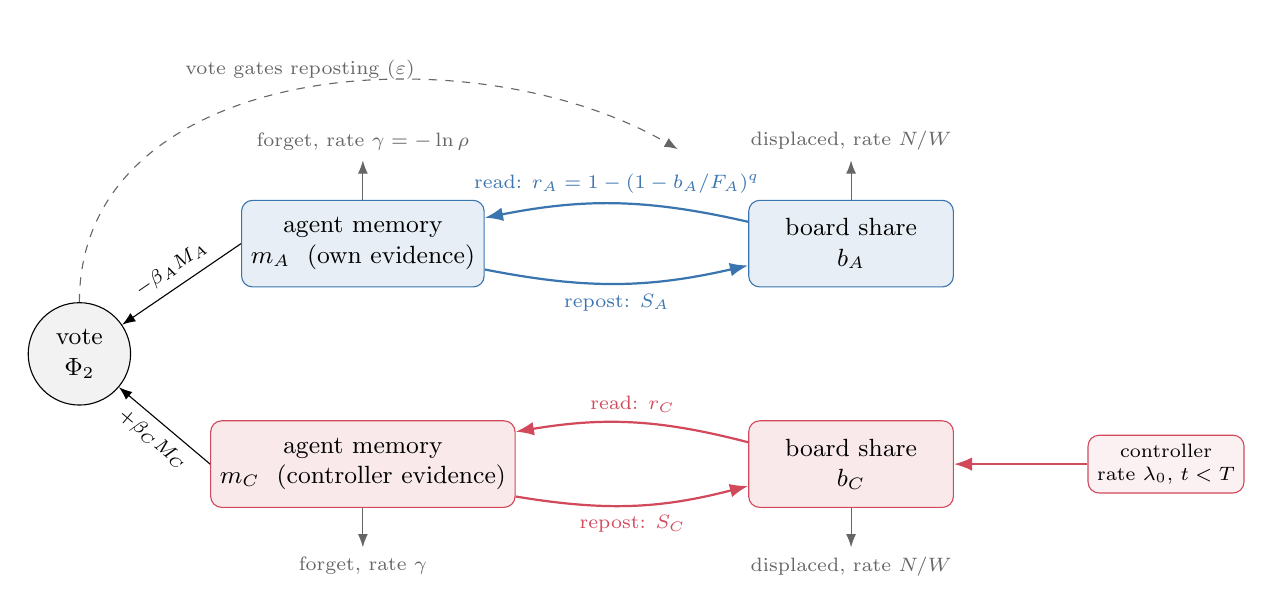
\begin{tikzpicture}[font=\small, >=Latex,
  res/.style={draw, rounded corners, minimum width=26mm, minimum height=11mm, align=center},
  lab/.style={font=\scriptsize, align=center}]
  \node[res, fill=cA!12, draw=cA] (mA) at (0,1.4) {agent memory\\ $m_A$ \ (own evidence)};
  \node[res, fill=cC!12, draw=cC] (mC) at (0,-1.4) {agent memory\\ $m_C$ \ (controller evidence)};
  \node[res, fill=cA!12, draw=cA] (bA) at (6.2,1.4) {board share\\ $b_A$};
  \node[res, fill=cC!12, draw=cC] (bC) at (6.2,-1.4) {board share\\ $b_C$};
  \node[draw, circle, fill=black!5, minimum size=13mm, align=center] (V) at (-3.6,0) {vote\\ $\Phi_2$};
  \node[draw=cC, rounded corners, fill=cC!8, align=center, font=\scriptsize] (ctrl) at (10.2,-1.4) {controller\\ rate $\lambda_0$, $t<T$};
  \draw[->, thick, cA] (bA) to[bend right=12] node[lab, above] {read: $r_A=1-(1-b_A/F_A)^q$} (mA);
  \draw[->, thick, cA] (mA) to[bend right=12] node[lab, below] {repost: $S_A$} (bA);
  \draw[->, thick, cC] (bC) to[bend right=12] node[lab, above] {read: $r_C$} (mC);
  \draw[->, thick, cC] (mC) to[bend right=12] node[lab, below] {repost: $S_C$} (bC);
  \draw[->, thick, cC] (ctrl) -- (bC);
  \draw[->] (mA.west) -- node[lab, above, sloped] {$-\beta_A M_A$} (V);
  \draw[->] (mC.west) -- node[lab, below, sloped] {$+\beta_C M_C$} (V);
  \draw[->, dashed, black!60] (V) to[out=90, in=150] node[lab, above] {vote gates reposting ($\varepsilon$)} (4.0,2.6);
  \draw[->, black!60] (mA.north) -- ++(0,0.5) node[lab, above] {forget, rate $\gamma=-\ln\rho$};
  \draw[->, black!60] (mC.south) -- ++(0,-0.5) node[lab, below] {forget, rate $\gamma$};
  \draw[->, black!60] (bA.north) -- ++(0,0.5) node[lab, above] {displaced, rate $N/W$};
  \draw[->, black!60] (bC.south) -- ++(0,-0.5) node[lab, below] {displaced, rate $N/W$};
\end{tikzpicture}
\caption{\textbf{The fact-flow model.} Facts of each class circulate between two reservoirs: agents' memories and the
board. Reading moves copies from the board to memory, and reposting moves them back. Forgetting and board turnover remove
copies. The controller injects controller facts until $T=30$. The vote depends on how much evidence of each kind an
agent holds, and the vote in turn affects what is reposted.}
\label{fig:model}
\end{figure}

\paragraph{Variables.} Each class $\alpha\in\{A,C\}$ has $F_\alpha$ interchangeable facts.
\begin{itemize}
\item $m_\alpha(t)$ is the probability that an agent holds a given class-$\alpha$ fact;
\item $M_\alpha=F_\alpha m_\alpha$ is the expected number of class-$\alpha$ facts an agent holds;
\item $b_\alpha(t)$ is the share of the readable board carrying class-$\alpha$ posts.
\end{itemize}
Agents act at rate 1 and read $q$ posts. Each remembered fact is forgotten at rate $\gamma=-\ln\rho$. The board turns
over at rate $N/W$. The controller posts at rate $\lambda(t)=\lambda_0$ for $t<T$, and 0 afterwards.

\paragraph{Equations.}
\begin{align}
\dot m_\alpha&=(1-m_\alpha)\,r_\alpha-\gamma\,m_\alpha,\qquad r_\alpha=1-\Big(1-\frac{b_\alpha}{F_\alpha}\Big)^{q},\label{eq:m}\\
\dot b_\alpha&=\frac NW\big(S_\alpha-b_\alpha\big)+\frac{\lambda(t)}{W}\big(u_\alpha-b_\alpha\big),\qquad u_C=1,\ u_A=0,\label{eq:b}\\
\Phi_2&=(1-z)\,\sigma(x),\qquad x=h_0+\beta_C M_C-\beta_A M_A,\qquad \sigma(x)=\frac1{1+e^{-x}},\label{eq:phi}\\
S_C&=\frac{w_C}{w_A+w_C+\kappa_0},\quad S_A=\frac{w_A}{w_A+w_C+\kappa_0},\nonumber\\
w_C&=\kappa_C M_C\big[\varepsilon+(1-\varepsilon)\Phi_2\big],\qquad w_A=\kappa_A M_A\big[\varepsilon+(1-\varepsilon)(1-\Phi_2)\big].\label{eq:S}
\end{align}
What each piece means:
\begin{itemize}
\item \textbf{Eq.~\eqref{eq:m}:} memory gains facts by reading and loses them by forgetting.
\item \textbf{Eq.~\eqref{eq:b}:} the board gains posts from agents and from the controller, and loses old ones by
  turnover.
\item \textbf{Eq.~\eqref{eq:phi}:} the probability of voting for the wrong answer $A2$ rises with controller evidence and
  falls with the agents' own evidence. $h_0$ sets the starting belief, $P(A2)=1/3$. $z$ is the chance of holding a
  complete proof of the correct answer, which forces $\Phi_2=0$ (Section~\ref{sec:proofs}; $z=0$ elsewhere).
\item \textbf{Eq.~\eqref{eq:S}:} agents repost facts of each class in proportion to how many they hold. The factor in
  brackets is the \emph{vote gating}:
  \begin{itemize}
  \item $\varepsilon=0$ is the plan's rule: only agents who believe $A2$ repost controller facts;
  \item $\varepsilon=1$ is neutral reposting, ignoring the vote.
  \end{itemize}
  $\varepsilon$ is the part of reposting eligibility that does not depend on the vote.
\end{itemize}

\paragraph{Observables.} The controlled arm has $\lambda_0>0$. The silent arm has $\lambda=0$ and $m_C=b_C=0$. Then
\begin{equation}
G=\Phi_2^{\rm controlled}(T)-\Phi_2^{\rm silent}(T),\qquad D(q_1\!\to\!q_2)=G(q_2)-G(q_1),\qquad
\delta(t)=\Phi_2^{\rm controlled}(t)-\Phi_2^{\rm silent}(t)\ \ (t>T).\label{eq:obs}
\end{equation}
After $T$ both arms follow one of four continuations:
\begin{itemize}
\item \emph{normal};
\item \emph{frozen board}: $b$ fixed, no posting;
\item \emph{no communication}: no reading, no posting;
\item \emph{controller facts removed}: $m_C=b_C=0$ at $T$, then normal.
\end{itemize}

\paragraph{Parameters} (set P0, chosen before any run): $N/W=0.5$, $F_A=16$, $F_C=4$, $\beta_A=\beta_C=0.5$,
$h_0=\ln\tfrac12$, $\kappa_A=\kappa_C=1$, $\kappa_0=0.2$, $\lambda_0=1$, $W=48$, $T=30$. Agents start with one own fact
each ($m_A=1/F_A$). The current best version has $\varepsilon=1$.

\section{Analytical results}
\begin{result}[frozen board]
With $b$ fixed, Eq.~\eqref{eq:m} is linear and
\begin{equation}m_\alpha\to m_\alpha^*=\frac{r_\alpha}{r_\alpha+\gamma}>0.\label{eq:frozen}\end{equation}
So the effect is kept indefinitely. This is the same form as the simulator's exact single-fact result from Phase~A.
\end{result}

\begin{result}[no communication, and a transient rise]
With no reading, $m_\alpha(T+s)=m_\alpha(T)e^{-\gamma s}$, so $x\to h_0$ in both arms and $\delta\to0$. Initially,
\begin{equation}\frac{d\delta}{ds}\Big|_{0}=-\gamma\Big[\sigma'(x_c)(x_c-h_0)-\sigma'(x_s)(x_s-h_0)\Big].\label{eq:bump}\end{equation}
This slope can be \emph{positive}. As everyone's evidence fades, both arms slide back toward the prior. The controlled
arm's belief in $A2$ then rises faster, because the agents' own evidence that held it down is fading. $\delta$ rises
before it decays (Fig.~\ref{fig:cont}, $\rho=0.75$). The simulator shows the same transient in its symmetric setups at
$\rho=0.75$. Here it arises without any proof.
\end{result}

\begin{result}[reading reversal: dose against sensitivity]
For a small controller effect, $G\approx\sigma'(x_s)\,\beta_C M_C$: the population's \emph{sensitivity} $\sigma'$ at the
silent operating point, times the controller's \emph{dose} $M_C$. Differencing in $q$,
\begin{equation}
D\approx\beta_C\,\sigma'(x_s)\Big[\underbrace{\Delta M_C}_{\text{dose}\ (+)}-\underbrace{(1-2\Phi_s)\,\beta_A\,M_C\,\Delta M_A}_{\text{sensitivity}\ (-\text{ if }\Phi_s<1/2)}\Big].\label{eq:reversal}
\end{equation}
Reading always raises the dose. It also adds the agents' own evidence $\Delta M_A$, which pushes the population away
from the tipping point, where the sigmoid is flatter. With short memory, $\Delta M_A$ is small and the dose wins:
$D>0$. With long memory, agents accumulate their own evidence, and the sensitivity loss wins: $D<0$.
\end{result}

\begin{result}[persistence threshold]
After the stop, linearise Eqs.~\eqref{eq:m}--\eqref{eq:b} for the controller class when it is rare:
$\dot m_C\simeq (q/F_C)\,b_C-\gamma m_C$ and $\dot b_C\simeq (N/W)\big(\kappa_C F_C g_C m_C/H-b_C\big)$, with
$g_C=\varepsilon+(1-\varepsilon)\Phi_2$ and $H=\kappa_A M_A g_A+\kappa_0$. The controller class can sustain itself if
and only if
\begin{equation}\boxed{\ \mathcal R_C=\frac{q\,\kappa_C\,g_C}{\gamma\,H}>1\ }\label{eq:R}\end{equation}
(the determinant changes sign; the trace is always negative). $N/W$ sets the speed, not the threshold. In the mean-field
model, "sustain" means a stable mixed state: $\delta$ settles to a plateau. A finite swarm would eventually lose it.
\end{result}

\section{Numerical demonstrations}
\subsection{The reading reversal}
\begin{figure}[h]
\centering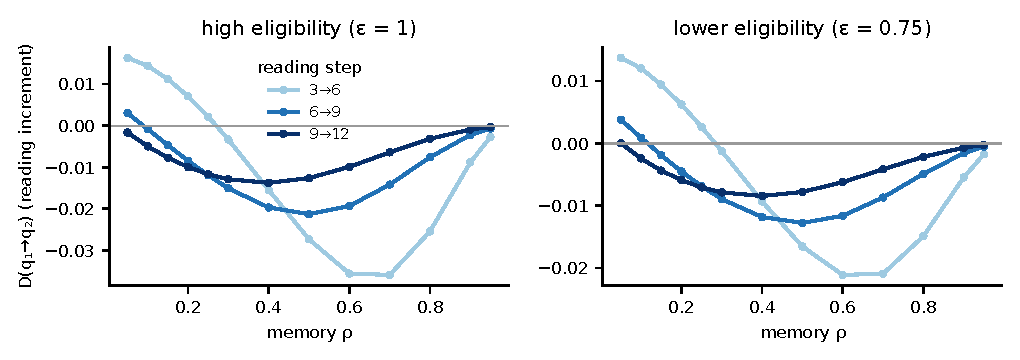
\includegraphics[width=\linewidth]{fig2_reversal.pdf}
\caption{\textbf{Reading reversal in the model} for two vote gatings. Above zero, reading more helps the controller;
below zero, it protects the swarm. The crossover moves to shorter memory as reading grows, as in the simulator.}
\label{fig:rev}
\end{figure}
\begin{figure}[h]
\centering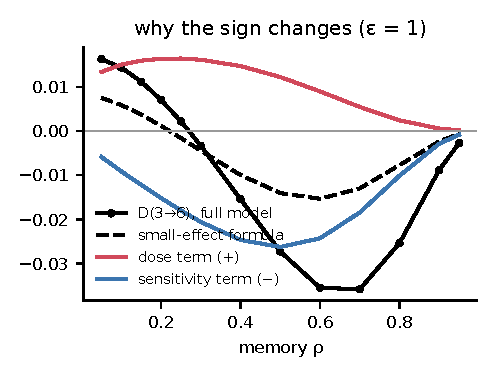
\includegraphics[width=0.5\linewidth]{fig3_dose_sensitivity.pdf}
\caption{\textbf{Why the sign changes} ($\varepsilon=1$): the full model's $D(3\to6)$, the small-effect formula
\eqref{eq:reversal}, and its dose and sensitivity terms. The formula has the right sign except where $D\approx0$, and the
size within a factor of about 2.}
\label{fig:mech}
\end{figure}
At P0 (with the plan's $\varepsilon=0$), $D(3\to6)=+0.003$ at $\rho=0.05$ and $-0.005$ at $\rho=0.5$. The crossover lies
between 0.2 and 0.3 for $3\to6$, between 0.1 and 0.2 for $6\to9$, and between 0.05 and 0.1 for $9\to12$. The reversal
survives 16 of 22 single-parameter changes (halving or doubling each). It fails when the agents' evidence per fact
$\beta_A$ is halved (positive everywhere) or doubled (negative everywhere), and when $h_0=0$. It does not need:
\begin{itemize}
\item proofs ($z=0$);
\item selective reposting (it holds at every $\varepsilon$);
\item few controller facts (it holds with $F_C=F_A$).
\end{itemize}
This last point contradicts the mechanism I had predicted in advance (the controller's few facts saturating in memory).

\subsection{Persistence and the four continuations}
\begin{table}[h]
\centering\small
\begin{tabular}{@{}lccccc@{}}
\toprule
vote gating $\varepsilon$ & 0 (plan) & 0.25 & 0.5 & 0.75 & 1 (neutral)\\
\midrule
reversal $3\to6$ & yes & yes & yes & yes & yes\\
retained $\delta(130)/\delta(30)$, $\rho=0.25$ & 0 & 0 & 0 & 0.32 & 0.65\\
retained, $\rho=0.75$ & 0 & 0 & 0.29 & 0.63 & 0.75\\
$\mathcal R_C$ at the stop, $\rho=0.25$ / $0.75$ & 0.20 / 0.03 & 0.57 / 0.66 & 0.96 / 1.33 & 1.37 / 2.03 & 1.79 / 2.76\\
\bottomrule
\end{tabular}
\caption{Persistence as a function of vote gating (P0 otherwise). Both phenomena hold for $\varepsilon\gtrsim0.75$.}
\label{tab:eps}
\end{table}
\begin{figure}[h]
\centering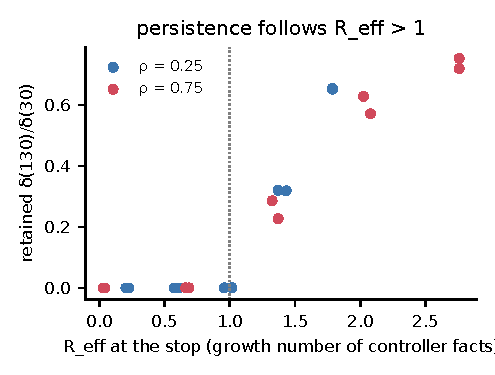
\includegraphics[width=0.48\linewidth]{fig4_threshold.pdf}
\caption{\textbf{Persistence follows the growth threshold \eqref{eq:R}.} Each point is one setting of the
revision-3 grid. The retained fraction is about zero when $\mathcal R_C<1$, and it rises above.}
\label{fig:thr}
\end{figure}
\begin{figure}[h]
\centering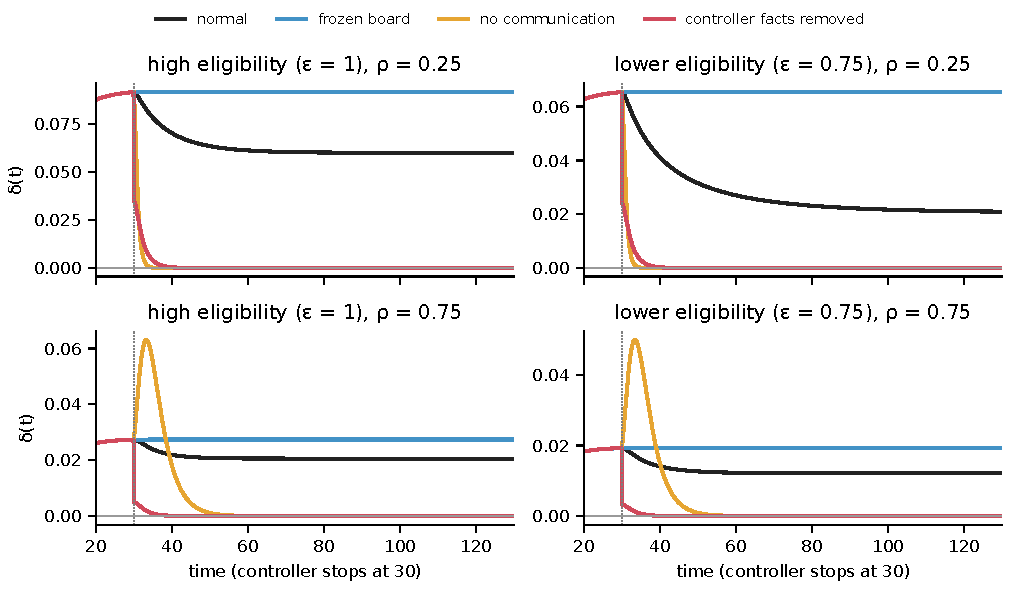
\includegraphics[width=\linewidth]{fig5_continuations.pdf}
\caption{\textbf{The four continuations after the stop} ($q=6$). The frozen board keeps the effect, no communication
removes it (with a transient rise at $\rho=0.75$), and removing the controller's facts removes it. Under normal
continuation the effect settles at a plateau whose height depends on $\varepsilon$.}
\label{fig:cont}
\end{figure}
\begin{figure}[h]
\centering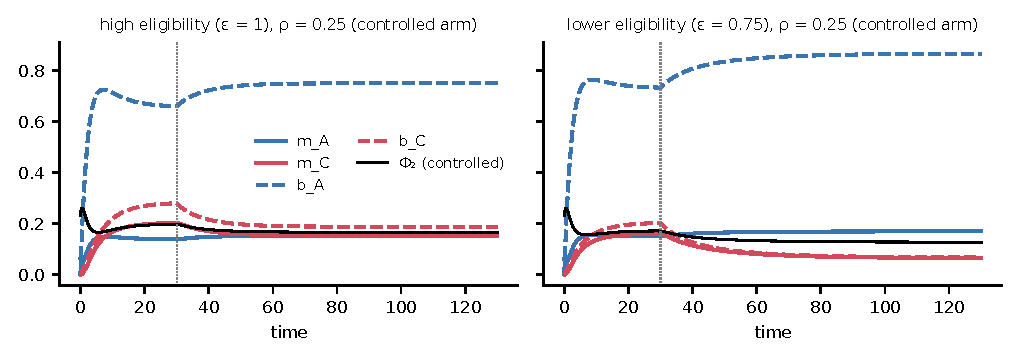
\includegraphics[width=\linewidth]{fig6_trajectories.pdf}
\caption{\textbf{Information currents} in the controlled arm ($\rho=0.25$): memory and board densities of both classes,
and the vote. With lower $\varepsilon$, controller facts lose board share after the stop.}
\label{fig:traj}
\end{figure}
Three findings (Table~\ref{tab:eps}, Figs.~\ref{fig:thr}--\ref{fig:traj}):
\begin{itemize}
\item \textbf{Tying reposting of controller facts to belief in the wrong answer undermines persistence.} With the plan's
  rule ($\varepsilon=0$), controller facts are reposted only by agents who already believe $A2$. At P0 those are few, so
  $\mathcal R_C\approx0.2$ and the effect is gone about 10 time units after the stop.
\item \textbf{A very strong reposting advantage instead flips the system.} With $\kappa_C/\kappa_A\ge4$, the controlled
  arm switches into a controller-dominated state and stays there (bistability). That is not the simulator's pattern, and
  it held together with the reversal at only one corner of the grid.
\item \textbf{Partly vote-independent reposting ($\varepsilon\gtrsim0.75$) gives both phenomena:} moderate, stable
  persistence whose level rises with $\varepsilon$.
\end{itemize}

\section{Proofs: the symmetric setups and Object Placements}
\label{sec:proofs}
\paragraph{Which setups the model describes.} The model has no task. With $z=0$ no proof can form, which describes the
no-proof setups. The symmetric setups differ by having proofs of the correct answer. The two tasks differ in how big and
how many those proofs are. In the symmetric setups, the smallest proof built from agents' facts has 6 facts in task003,
with 12 such proofs, and 3 facts in Object Placements, with 2 such proofs. These counts come from the worlds, not from a
fit. We added the plan's single proof variable
\begin{equation}z=Z(m_A)=1-\big(1-m_A^{\ell}\big)^{P},\qquad (\ell,P)=(6,12)\ \text{task003-like},\quad(3,2)\ \text{Object-Placements-like},\label{eq:z}\end{equation}
the chance that an agent holds at least one complete proof, treating the facts of a proof as held independently.

\begin{figure}[h]
\centering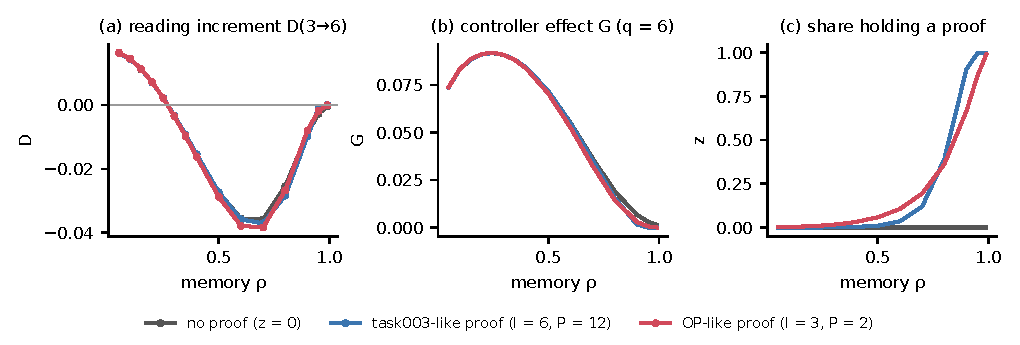
\includegraphics[width=\linewidth]{fig7_proofs.pdf}
\caption{\textbf{Adding proofs} ($\varepsilon=1$). (a) The reversal is unchanged and the crossover does not move. (b) The
effect goes to zero at long memory. (c) In the model, proofs form only at very long memory, after the crossover.}
\label{fig:proofs}
\end{figure}
Against the expectations written before the run:
\begin{itemize}
\item \textbf{The reversal survives with proofs: met.}
\item \textbf{Proofs send $G$ to 0 at long memory: met.} At $\rho=0.99$, $G$ is 0.0014 without proofs and 0 with either
  proof shape. The simulator's symmetric $G$ is also 0 at $\rho=1$.
\item \textbf{Proofs move the crossover to shorter memory, more so for 3-fact proofs: not met.} The crossover stays at
  0.25--0.3. In the simulator, the symmetric crossover is lower than the no-proof one in both tasks, and lower in Object
  Placements than in task003.
\end{itemize}

The reason is in Fig.~\ref{fig:proofs}(c). In the model, the share of agents holding a proof is only 0.01 (task003-like)
and 0.06 (Object-Placements-like) at $\rho=0.5$, so proofs appear only after the crossover. Two simplifications cause
this:
\begin{itemize}
\item each agent fact is held with a low probability, because 16 facts compete for reading;
\item Eq.~\eqref{eq:z} treats the facts of a proof as held independently.
\end{itemize}
On stored simulator data, the ChatGPT agent showed that independent products \emph{under-estimate} how often the facts
of a proof are held together, by factors of 1.8--2.6, because one read can bring several of them at once. So the missing
ingredient is this \emph{co-retention}. With it, proofs would form at shorter memory, and Object
Placements' smaller proofs should move the crossover more than task003's.

\section{Comparison with the simulator (qualitative, no fitting)}
\begin{table}[h]
\centering\small
\resizebox{\linewidth}{!}{%
\begin{tabular}{@{}llll@{}}
\toprule
feature & simulator & model & agreement\\
\midrule
reversal: $D>0$ at short memory, $<0$ at long memory & yes, all four setups & yes & yes\\
crossover moves to shorter memory as $q$ grows & yes & yes & yes\\
reversal without any possible proof & yes (no-proof setups) & yes ($z=0$) & yes\\
symmetric crossover lower than no-proof (more so in OP) & yes & no (crossover unchanged) & no\\
frozen board keeps the effect & yes & yes, exactly & yes\\
no communication: effect vanishes within a few memory lifetimes & yes & yes & yes\\
transient rise when communication stops (long memory) & yes (symmetric $\rho=0.75$) & yes & yes, different cause\\
removing controller facts removes most of the effect & yes, small residual & yes, no residual & partly\\
normal continuation: task003 flat, OP fades & 1.0 / 0.33--0.67 over 100 units & plateau 0.65--0.75 / 0.32--0.63 within 5--9 units & levels yes, timing no\\
size of $G$ & 0.1--0.45 & 0.02--0.09 & no (not a target)\\
\bottomrule
\end{tabular}}
\caption{What the model reproduces. "OP" = Object Placements. For the normal-continuation row the model's two values are
$\varepsilon=1$ and $\varepsilon=0.75$.}
\label{tab:cmp}
\end{table}

\section{Path taken (all revisions single changes, logged before running)}
\begin{enumerate}
\item \textbf{Stage A, P0:} reversal present and robust; my predicted mechanism was wrong. The chain-rule split found
  dose against sensitivity.
\item \textbf{Stage D, P0:} with the plan's reposting rule, no persistence ($\mathcal R_C\approx0.2$). Neutral
  reposting keeps 65--75\%.
\item \textbf{Revision 1:} stronger controller facts. The reversal is kept; still no persistence.
\item \textbf{Revision 2:} a reposting advantage for controller facts. This gives bistability (lock-in), and both
  phenomena at only one corner.
\item \textbf{Revision 3:} partly vote-independent reposting ($\varepsilon$). Both phenomena hold for
  $\varepsilon\gtrsim0.75$; persistence follows $\mathcal R_C>1$.
\item \textbf{Stage C:} proofs with task-derived sizes. Two of four expectations met; the crossover does not move.
\end{enumerate}

\section{Next steps}
\label{sec:next}
\begin{enumerate}
\item \textbf{Proofs with co-retention.}
  \begin{itemize}
  \item \emph{What:} replace the independent product in Eq.~\eqref{eq:z} by a quantity that follows how often a proof's
    facts are held \emph{together}.
  \item \emph{How:} a combination's chance of being held grows when one read brings several of its facts at once. The
    ChatGPT agent's equations give exactly this for a fixed board. For our two-class model, the minimal version is one
    extra variable $h_\ell(t)$, the chance of holding all $\ell$ facts of a proof. It obeys a small set of equations
    driven by the same reading and forgetting rates.
  \item \emph{Test, fixed in advance:} does the crossover then move to shorter memory with proofs, and more for 3-fact
    proofs than for 6-fact ones?
  \item \emph{Why first:} it is the one setup difference the model does not yet reproduce, and the only one with an
    identified cause.
  \end{itemize}
\item \textbf{A formula for where the crossover sits.}
  \begin{itemize}
  \item \emph{What:} the $\rho$ at which the dose and sensitivity terms of Eq.~\eqref{eq:reversal} balance, as a
    function of $q$.
  \item \emph{How:} at the stop time, memory densities are close to the steady state of Eq.~\eqref{eq:m}. In the limits
    of short memory ($m\approx r/\gamma$) and long memory ($m\to1$), the two terms can be written in closed form. Setting
    them equal gives $\rho^*(q)$.
  \item \emph{Test:} does $\rho^*(q)$ fall as $q$ grows, as in Fig.~\ref{fig:rev} and in the simulator? Which parameters
    set it?
  \item \emph{Why:} it would turn ``the crossover moves with $q$'' from an observation into a derived prediction.
  \end{itemize}
\item \textbf{A minimal finite-swarm version.}
  \begin{itemize}
  \item \emph{What:} make a handful of representative facts finite: integer numbers of holders and board copies, which
    can reach zero.
  \item \emph{Why:} two mismatches in Table~\ref{tab:cmp} are finite-size effects in the simulator (Phase~C1):
    \begin{itemize}
    \item the lasting residual after removal, caused by extinction of agents' own facts;
    \item the slow fading of persistence, caused by selection removing the controller's facts one by one.
    \end{itemize}
    A two-class mean field can show neither.
  \item \emph{Test:} does the finite version give a nonzero residual after removal, and a decline over tens of time
    units instead of a plateau within 5--9?
  \end{itemize}
\item \textbf{Two qualitative checks on stored simulator data.}
  \begin{itemize}
  \item \emph{Sensitivity:} in the simulator's memories, does adding one controller fact change $P(A2)$ less for agents
    who hold more of their own facts? If not, the dose-against-sensitivity explanation does not carry over.
  \item \emph{Vote gating:} do agents who do \emph{not} vote for $A2$ repost controller facts, and more often in task003
    than in Object Placements? This would support reading $\varepsilon$ as the task property behind persistent against
    fading effects.
  \end{itemize}
  Both use data we already have.
\end{enumerate}

\end{document}
